\section{Modelling of the Entire System}
To be able to produce vibrations using the magnetic field produced by the coil we need to introduce to the system an object that can react to the magnetic field. As the magnetic field of the coil is very feeble we can use as the object Neodymium magnets, these are permanent magnets with a very strong internal magnetic field for their size.
Using small ones and with the right pole facing the coil (same polarity as the generated magnetic field) it will be able to repel them and make them vibrate.
Then to constrain the motion of the magnet and make it only move in the z-axis we have to add to the system a flexible membrane.

We can now model the entire system using a bond graph, as shown in figure \ref{fig:bond-graph}.
\begin{figure}
    \centering
    \resizebox{.9\linewidth}{!}{\begin{tikzpicture}
    \begin{scope}[every node/.style={bgelement}]
    \node (Se) at (0,0) {Se: Power Supply};
    \node[right=1 of Se] (i) {1: elec};
    \node[above=1 of i] (Iel) {I: L\textsubscript{coil}};
    \node[below=1 of i] (Rel) {R: R\textsubscript{coil}};
    \node[right=1 of i] (CI) {CI: Coil+Magnet};
    \node[right=1 of CI] (w1) {1: mech};
    \node[above=1 of w1] (Cm) {C: C\textsubscript{membrane}};
    \node[below=1 of w1] (Im) {I: M\textsubscript{magnet} + M\textsubscript{finger}};
    \node[right=1 of w1] (v) {0};
    \node[above=1 of v] (w2) {1};
    \node[above=1 of w2] (Rdf) {R: Rd\textsubscript{finger}};
    \node[right=1 of w2] (Cf) {C: $\frac{1}{Ks_{finger}}$};
    \node[right=1 of v] (Sfa) {S\textsubscript{finger}};
    \end{scope}
    \draw[bonds]
    (Se) edge [e_out] (i)
    (i) edge [e_in] (Iel)
    edge [e_in] (Rel)
    edge [e_in] (CI)
    (CI) edge [e_in] (w1)
    (w1) edge [e_out] (Cm)
    edge [e_in] (Im)
    (w1) edge [e_in] (v)
    (v) edge [e_in] (w2)
    (w2) edge [e_in] (Rdf)
    (w2) edge [e_in] (Cf)
    (Sfa) edge [e_out] (v);
\end{tikzpicture}
    } % TODO: Da fare bene
    \caption{Bond graph of the coil-magnet-membrane system.}
    \label{fig:bond-graph}
\end{figure}

In the next subsections, we will analyze the physical laws that govern the behavior of the system and how to model them to create this bond graph.

% -- Subsection 5.1
\subsection{Neodynium magnets (magnetic strength wrt class and dimensions)}
Neodymium magnets are a type of rare-earth magnet, they are the strongest type of permanent magnets made commercially.
They are made of an alloy of neodymium, iron, and boron and their \textbf{strength depends on the percentage of neodymium} in the alloy and on its crystalline structure.
They are classified based on their maximum energy product, which is the maximum amount of energy that can be stored in a magnet. Modern neodymium magnets start from N35 and go up to N52 (even N55), the higher the number the stronger their magnetic field.

\begin{samepage}
    Considering a cylindrical magnet with a radius $R_M$ and a thickness $t$ we can calculate the magnetic field generated by it at a distance $z$ from a pole surface using the formula \cite{Magnetic_field_perm_magnet}:
    \nopagebreak

    \begin{equation}
        B_M(z) = \frac{B_r}{2} \left( \frac{t+z}{\sqrt{R_M^2+(z+t)^2}} - \frac{z}{\sqrt{R_M^2+z^2}} \right) 
        \label{eq: Magnetic_field_perm_magnet}
    \end{equation}
    \nopagebreak

    Where: 
    \begin{itemize}
        \item $B_r$ is the remanence of the magnet [T]
        \item $R_M$ is the radius of the magnet [m]
        \item $t$ is the thickness of the magnet [m]
        \item $z$ is the distance from a pole surface of the magnet [m]
    \end{itemize}
\end{samepage}
    
\begin{samepage}
    The remanence of a magnet is the magnetic field that remains in the magnet after the external magnetic field is removed and depends on the N grade of the magnet.
    \nopagebreak

    \begin{table}[H]
        \centering
        \resizebox{.6\linewidth}{!}{
            \begin{tabular}{|l | l l|} % <-- Alignments: 1st column left, 2nd column left
    \hline
    \rowcolor{black} {\color{white} Goudsmit Grade} & \multicolumn{2}{|c|}{\color{white} Remanence $B_r\, [mT]$} \cr
    \hline
     & \quad min value & \quad typical value \cr
    \hline
    N35 & \quad 1170 & \quad 1210 \cr
    \hline
    N38 & \quad 1220 & \quad 1260 \cr
    \hline
    N40 & \quad 1260 & \quad 1290 \cr
    \hline
    N42 & \quad 1290 & \quad 1320 \cr
    \hline
    N45 & \quad 1320 & \quad 1370 \cr
    \hline
    N48 & \quad 1370 & \quad 1420 \cr
    \hline
    N50 & \quad 1400 & \quad 1460 \cr
    \hline
    N52 & \quad 1420 & \quad 1470 \cr
    \hline
\end{tabular} % TODO: Fixare sta merda

        }
        \caption{Magnetic field remanence of different N grade neodymium magnets.}
        \label{tab: magnet_grades}
    \end{table}
\end{samepage}


% -- Subsection 5.2
\subsection{Magnetic force between magnet and coil}
To calculate the magnetic repulsion force between the coil and a permanent magnet we consider them aligned with their centers coinciding on the z-axis.
\begin{figure}
    \centering
    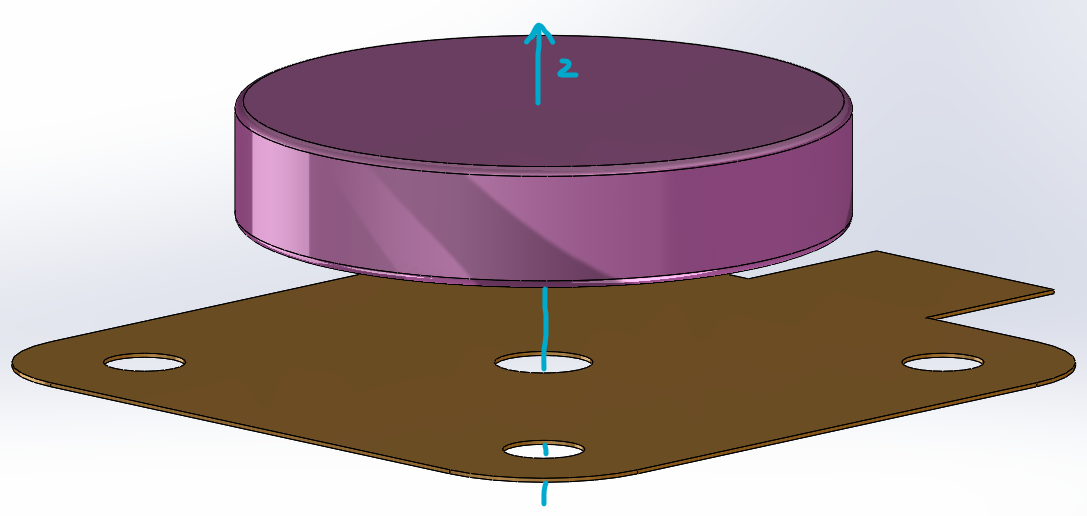
\includegraphics[scale=0.4]{Chapters/Chapter2/Modelling_of_Entire_System/Figures/coil_magnet.png} % TODO: Make a better image
    \caption[Coil-Magnet position]{Coil and magnet position in space.}
    \label{fig:Coil-Magnet position}
\end{figure}

The force between a magnet and a coil can be calculated using the magnetic field generated by the coil and magnet.
Knowing their closed-form expression we can calculate the force using this formula:
\begin{equation}
    F = \nabla (\overrightarrow{m_M} \cdot \overrightarrow{B_C}) % TODO: trovare fonte migliore di https://en.wikipedia.org/wiki/Magnetic_levitation
\end{equation}

Where: 
\begin{itemize}
    \item $\overrightarrow{m_M}$ is the magnetic moment of the magnet [A/m]
    \item $\overrightarrow{B_C}$ is the magnetic field generated by the coil [T]
\end{itemize}

The magnetic momentum of the magnet is defined as:
\begin{equation}
    \overrightarrow{m_M} = 
    \begin{pmatrix}
        0 & 0 & \frac{B_M(z)}{\mu}
    \end{pmatrix}
\end{equation}

Where:
\begin{itemize}
    \item $B_M(z)$ is the magnetic field generated by the permanent magnet [T]
    \item $\mu$ is the magnetic permeability of the medium [H/m]
\end{itemize}

We can calculate the magnetic field generated by the coil at a distance using equation \ref{eq:Spiral_magn_field_dist} (considering our coil as two in parallel) and the magnetic field generated by a cylindrical magnet at a distance $z$ using equation \ref{eq:Magnetic_field_perm_magnet}.

Doing the calculations, the resulting force in function of the distance $z$ is given by:
\begin{equation}
    F = \frac{ B_r I N R_C^2 \left(\frac{1}{\sqrt{\sigma_1}} - \frac{1}{\sqrt{\sigma_2}} + \frac{z^2}{\sigma_2^{3/2}} - \frac{2(t+z)^2}{2\sigma_1^{3/2}}\right)}{2\sigma_3^{3/2}} + B_C(I) \cdot \frac{3z \left(\frac{z}{\sqrt{\sigma_2}} - \frac{t+z}{\sqrt{\sigma_1}}\right)}{2\sigma_3}
\end{equation}
Where:
\begin{itemize}
    \item $N$ is the number of spires of a one-layer coil
    \item $I$ is the current flowing through the coil [A]
    \item $B_C$ is the coil magnetic field calculated as in \ref{eq:Spiral_magn_field_dist} [T]
    \item $R_C$ is the coil average radius ($r'$ in equation \ref{eq:Spiral_magn_field_dist}) [m]
    \item $\sigma_1 = R_M^2 + (t+z)^2$
    \item $\sigma_2 = R_M^2 + z^2$
    \item $\sigma_3 = R_C^2 + z^2$    
\end{itemize}

So we can model the coil-magnet system as a \textbf{Transducer} element that converts the current flowing through the coil into a force acting on the magnet.
\begin{equation}
    B_C(z, I) = \frac{\mu N I R_C^2}{2(R_C^2+z^2)^\frac{3}{2}} \rightarrow B_C(q, i) = \frac{1}{2} L(q) i
\end{equation}

\begin{figure}
    \centering
    \resizebox{.9\linewidth}{!}{\begin{tikzpicture}
    \begin{scope}[every node/.style={bgelement}]
    \node (start) at (0,0) {};
    \node[right=1 of start] (CI) {CI: Coil+Magnet};
    \node[right=1 of CI] (end) {};
    \end{scope}
    \draw[bonds]
    (start) edge [e_in, flow={i}, effort={V}] (CI)
    (end) edge [e_in, flow={v}, effort={F}] (CI);
\end{tikzpicture}
    }
    \caption{Coil-Magnet Transducer bond graph.}
    \label{fig:Coil-Magnet Transducer}
    \begin{equation}
        F(q, i) = \frac{1}{2} \frac{d \left(L(q) \cdot m_M(q) \right)}{dq} i
    \end{equation}
    \begin{equation}
        \lambda = L(q) i
    \end{equation}
\end{figure}


% -- Subsection 5.3
\subsection{Membrane-magnet system}
The magnet needs to be suspended to allow it to move freely only on the z-axis, to achieve this we need a structure that constrains the lateral motion of the magnet and needs to also be able to vibrate freely with it.
To do this we can use a flexible membrane that can deform under the magnetic field generated by the coil and the magnet. 

As an example, we will analyze the membrane structure of the last type of prototype we implemented \ref{sec: Flexible_Mat_Prototypes}
\begin{figure}
    \centering
    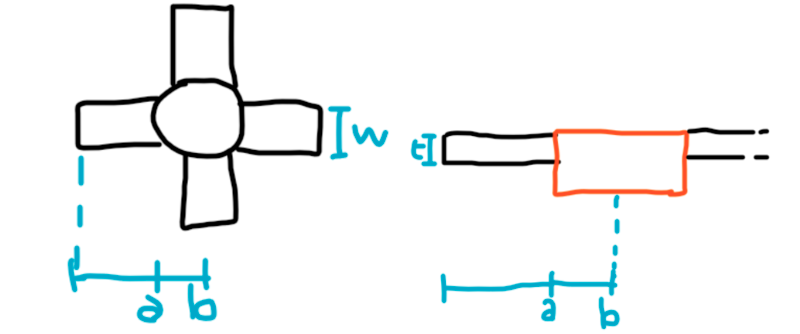
\includegraphics[scale=0.4]{Chapters/Chapter2/Modelling_of_Entire_System/Figures/membrane.png} % TODO: Change image with svg
    \caption[Membrane structure]{Membrane structure of the last prototype.}
    \label{fig: Membrane structure}
\end{figure}

This membrane is a simple Celtic-cross structure made of thin silicone integrated with the entire structure of the device,
the membrane is built with a central cylindrical chamber used to trap the magnet in the center of the cross.
\begin{figure}
    \centering
    \resizebox{.9\linewidth}{!}{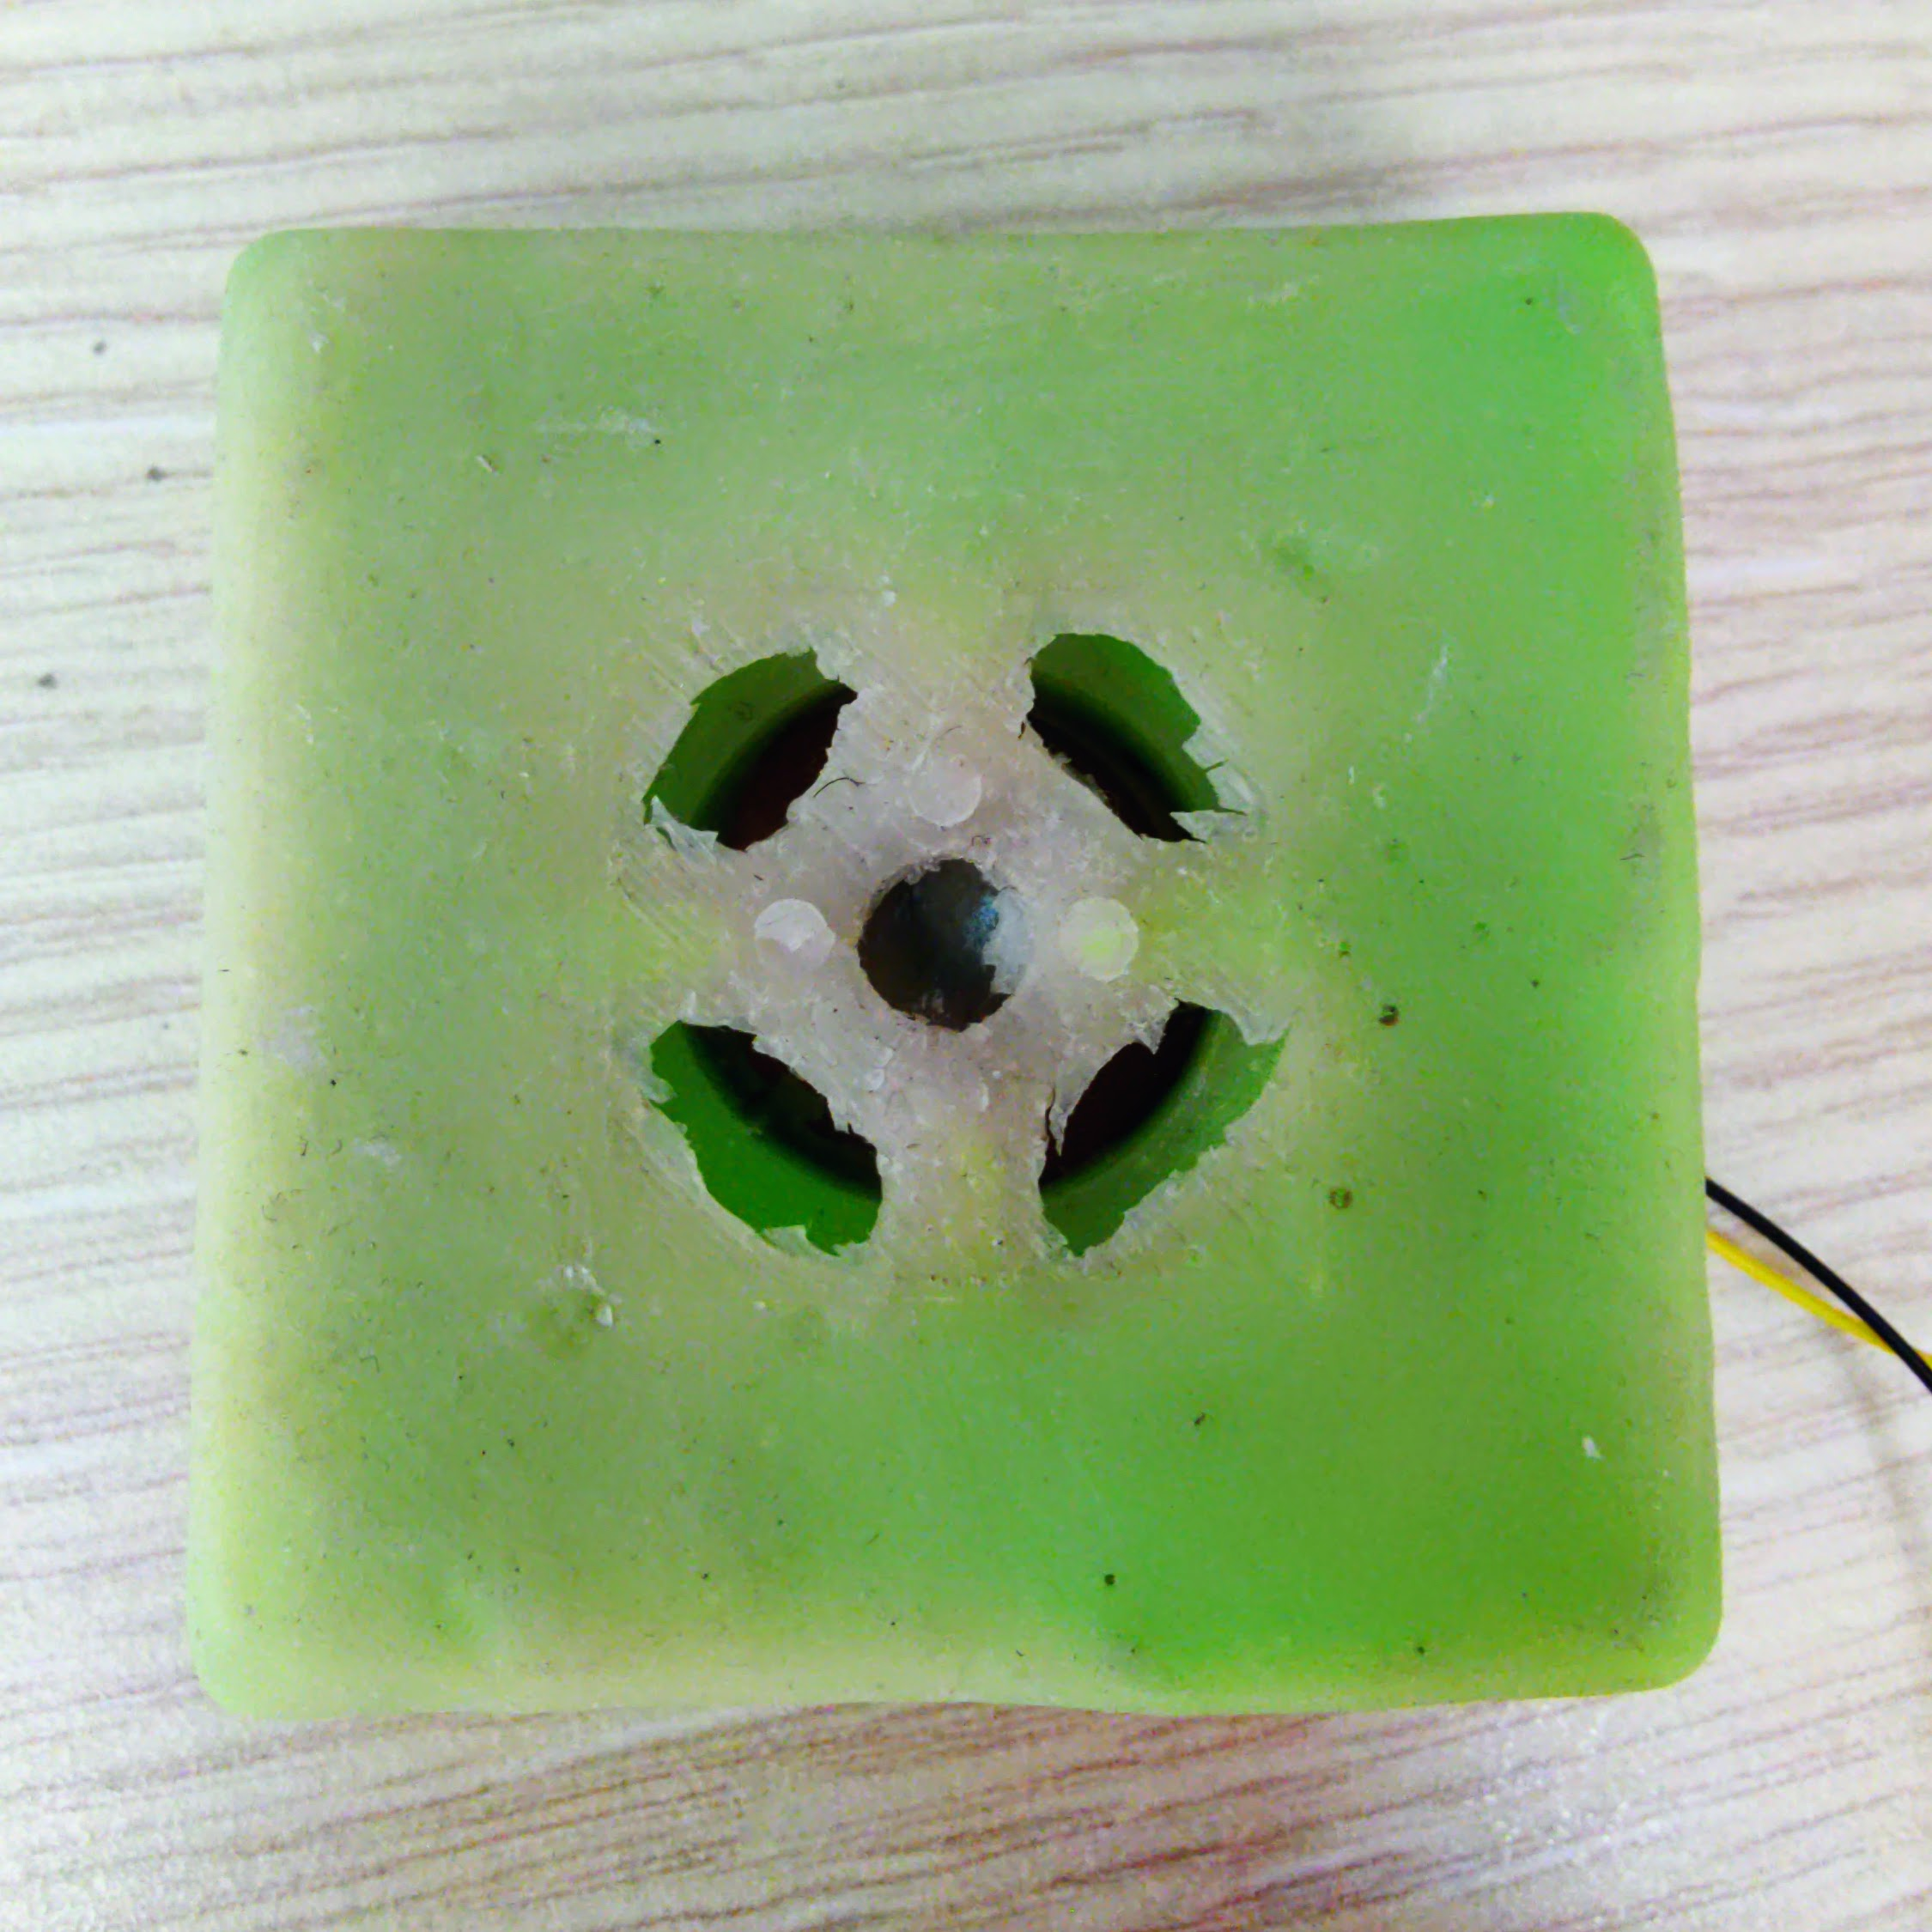
\includegraphics{Chapters/Chapter2/Modelling_of_Entire_System/Figures/Flexible_mat_small_top.jpg}}
    \caption[Membrane mat]{Membrane of the last prototype with the magnet trapped in the center.}
    \label{fig: Membrane trap}
\end{figure}

The membrane can be modeled as a mass-spring-damper system.
\begin{figure}
    \centering
    \resizebox{.9\linewidth}{!}{
        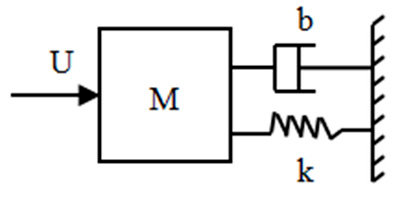
\includegraphics[scale = 0.6]{Chapters/Chapter2/Modelling_of_Entire_System/Figures/membrane_mech_model.png}
        \begin{tikzpicture}
    \begin{scope}[every node/.style={bgelement}]
    \node (start) at (0,0) {};
    \node[right=1 of start] (w) {1: Mech};
    \node[above=1 of w] (Cm) {C: $\frac{1}{ks_{membr}}$};
    \node[below=1 of w] (Rm) {R: b\textsubscript{membr}};
    \node[right=1 of w] (Im) {I: M\textsubscript{magnet}};
    \end{scope}
    \draw[bonds]
    (start) edge [e_in, flow={i}, effort={V}] (w)
    (w) edge [e_out] (Cm)
    (w) edge [e_in] (Rm)
    (w) edge [e_in] (Im);
\end{tikzpicture}    
    }
    \caption{Bond graph of the membrane-magnet system.}
    \label{fig: Membrane bond graph}
\end{figure}

\subsubsection{Membrane stiffness}
The membrane stiffness can be calculated using Young's modulus of the material and the geometry of the membrane.
Each arm of the cross can be considered as a cantilever beam, the stiffness of a cantilever beam can be calculated as:
\begin{equation}
    ks = \frac{3 E I_x}{L^3}
\end{equation}
Where:
\begin{itemize}
    \item $ks$ is the stiffness of the membrane's arm [N/m]
    \item $E$ is the Young's modulus of the material [Pa]
    \item $I$ is the second moment of inertia of the arm [m\textsuperscript{4}]
    \item $L$ is the length of the arm [m]
\end{itemize}

The arm can be simplified as a parallelepiped with a rectangular section, and the second moment of inertia on x can be calculated as:
\begin{equation}
    I_x = \frac{w t^3}{12}
\end{equation}
Where:
\begin{itemize}
    \item $I_x$ is the second moment of inertia on the x-axis [m\textsuperscript{4}]
    \item $w$ is the width of one membrane arm as in figure \ref{fig: Membrane structure}[m]
    \item $t$ is the thickness of the membrane as in figure \ref{fig: Membrane structure}[m]
\end{itemize}

\begin{figure}
    \centering
    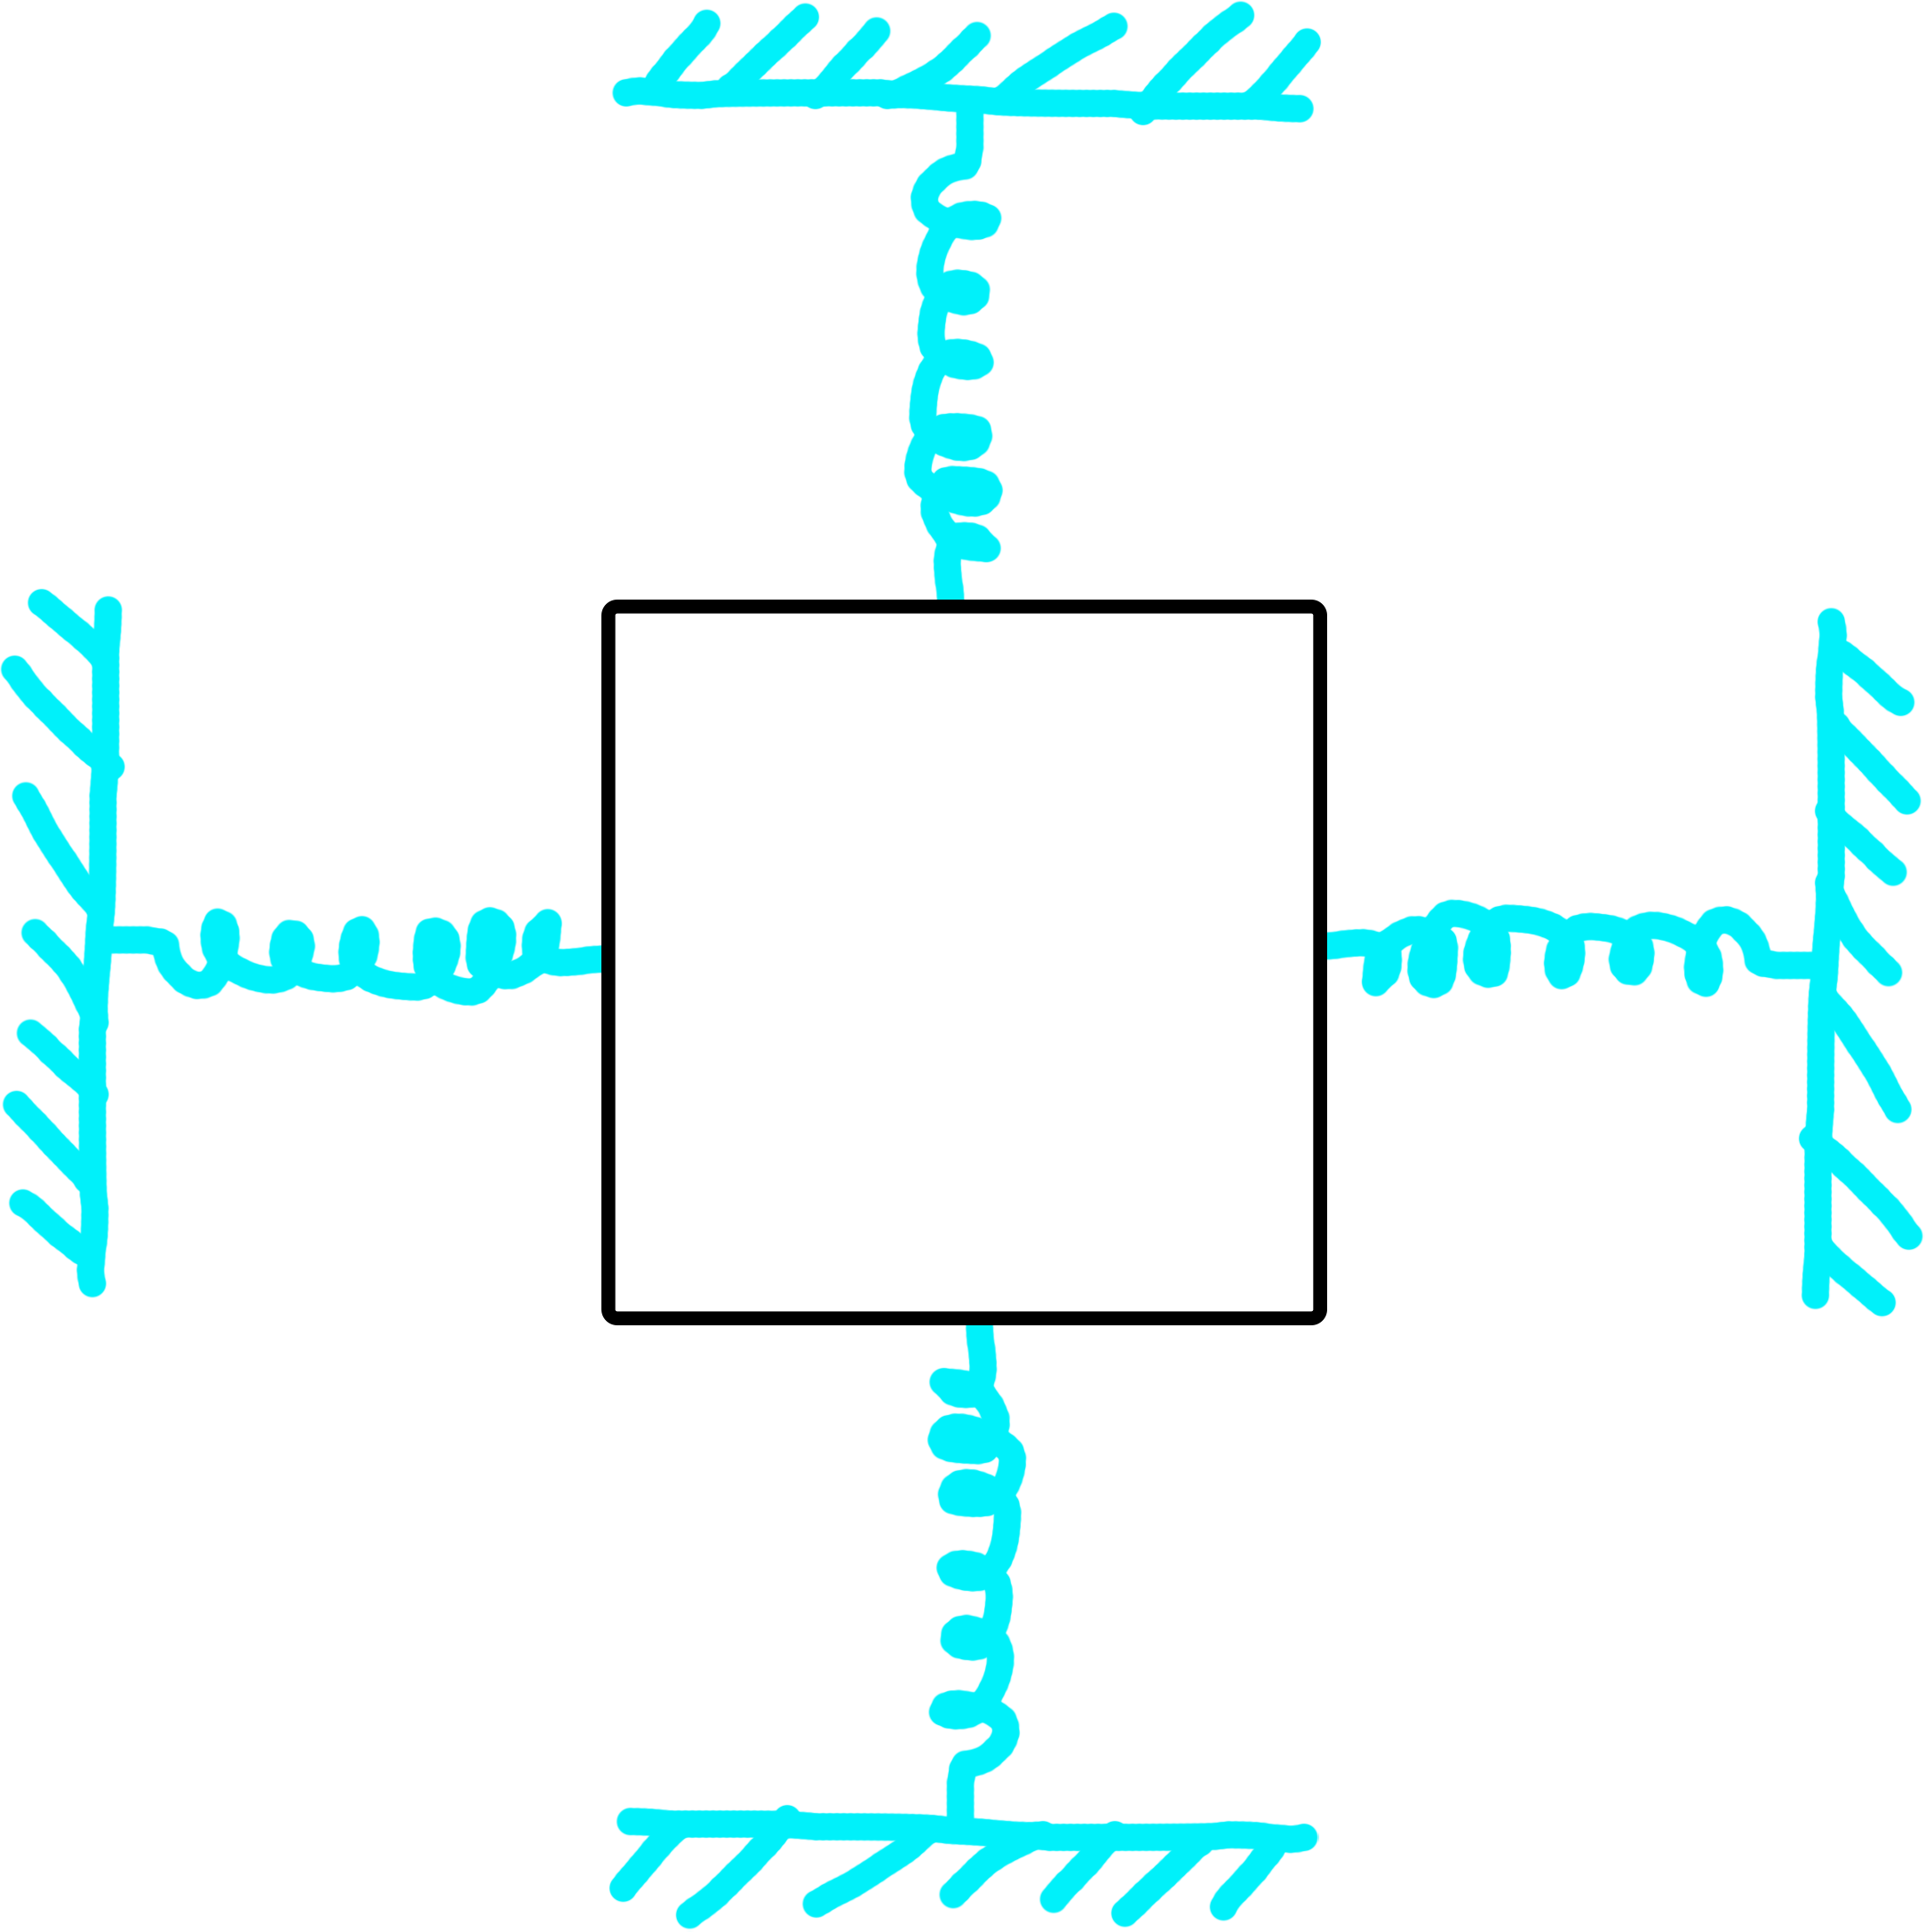
\includegraphics[scale=0.4]{Chapters/Chapter2/Modelling_of_Entire_System/Figures/4_arms_springs.png} % TODO: Change image with svg
    \caption{Membrane arms parallel springs.}
    \label{fig: Membrane springs}
\end{figure}
Then we can consider the 4 arms as 4 springs in parallel, the total stiffness of the membrane can be calculated as:
\begin{equation}
    ks_{membr} = 4 ks
\end{equation}


\subsubsection{Membrane damping}
The damping for a cantilever beam is neglectable, so we can remove the resistive component from the mechanical model.
\begin{figure}
    \centering
    \resizebox{.9\linewidth}{!}{
        \begin{tikzpicture}
    \begin{scope}[every node/.style={bgelement}]
    \node (start) at (0,0) {};
    \node[right=1 of start] (w) {1: Mech};
    \node[above=1 of w] (Cm) {C: $\frac{1}{ks_{membr}}$};
    \node[right=1 of w] (Im) {I: M\textsubscript{magnet}};
    \end{scope}
    \draw[bonds]
    (start) edge [e_in, flow={i}, effort={V}] (w)
    (w) edge [e_out] (Cm)
    (w) edge [e_in] (Im);
\end{tikzpicture}    
    }
    \caption{Final mechanical bond-graph of the membrane and magnet.}
    \label{fig: Membrane bond graph without damping}
\end{figure}



% -- Subsection 5.4
\subsection{Finger grasping model}
At last, we have also to model the finger grasping the device, we can derive the model from the one used in \cite{Finger_grasping_model} for the human finger.

\begin{figure}
    \centering
    \resizebox{.9\linewidth}{!}{
        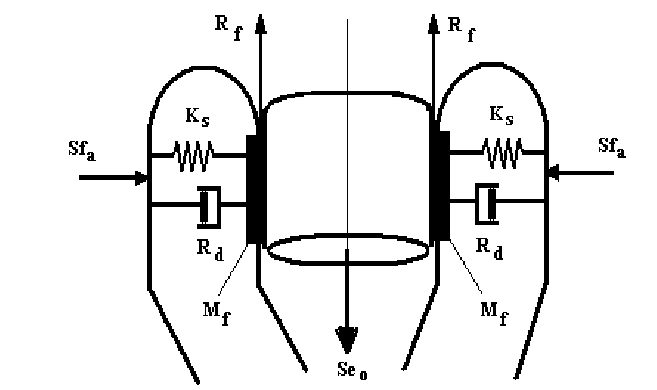
\includegraphics{Chapters/Chapter2/Modelling_of_Entire_System/Figures/Model-of-two-soft-fingers-grasping-the-object.png}
    }
    \caption{Model of two soft fingers grasping the object.}
    \label{fig: Finger grasping model}
\end{figure}

This model describes two fingers grasping an object, for our case, we can simplify it to a single finger grasping the device.
Also, we can neglect the friction between the finger and the device as the device will be tested positioned on a flat surface with only the finger touching it from above.
\begin{figure}
    \centering
    \resizebox{.9\linewidth}{!}{
        \begin{tikzpicture}
    \begin{scope}[every node/.style={bgelement}]
        \node (start) at (0,0) {};
        \node[right=1 of start] (w1) {1};
        \node[above=1 of w1] (Mf) {I: M\textsubscript{f}};
        \node[right=1 of w1] (v) {0};
        \node[above=1 of v] (w2) {1};
        \node[above=1 of w2] (Rdf) {R: Rd\textsubscript{f}};
        \node[right=1 of w2] (Cf) {C: $\frac{1}{Ks_{f}}$};
        \node[right=1 of v] (Sfa) {Sf\textsubscript{a}};
    \end{scope}
    \draw[bonds]
    (start) edge [e_out, flow={v}, effort={F}] (w1)
    (w1) edge [e_out] (Mf)
    (w1) edge [e_in] (v)
    (v) edge [e_in] (w2)
    (w2) edge [e_in] (Rdf)
    (w2) edge [e_in] (Cf)
    (Sfa) edge [e_out] (v);
\end{tikzpicture}
    }
    \caption{Bond graph of the finger grasping model.}
    \label{fig: Finger grasping bond graph}
\end{figure}
